\documentclass[border=6pt]{standalone}
\usepackage{tikz}
\usetikzlibrary{arrows.meta,positioning,calc,fit,backgrounds}
\usepackage[T1]{fontenc}
\usepackage{lmodern}
\usepackage{microtype}
\usepackage{amssymb}

\definecolor{combblue}{RGB}{66,133,244}
\definecolor{weightgreen}{RGB}{52,168,83}
\definecolor{sharedgray}{RGB}{120,120,120}
\definecolor{lgkkpurple}{RGB}{142,68,173}
\definecolor{lightbg}{RGB}{245,245,250}
\definecolor{lightgreen}{RGB}{240,250,240}

\begin{document}
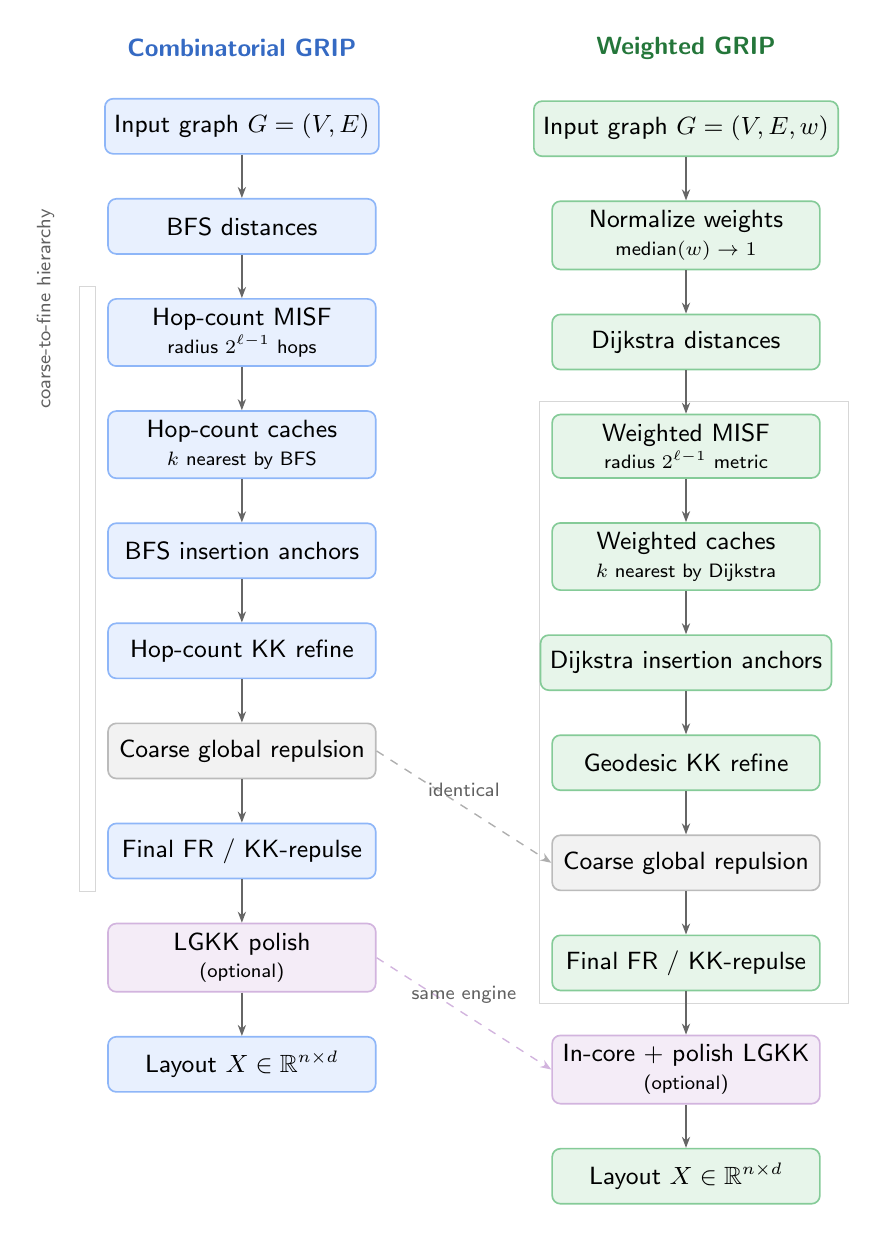
\begin{tikzpicture}[
    node distance=0.55cm and 2.8cm,
    box/.style={
      draw, rounded corners=3pt, minimum width=3.4cm,
      minimum height=0.7cm, align=center, font=\small\sffamily,
      line width=0.6pt
    },
    combbox/.style={box, fill=combblue!12, draw=combblue!60},
    wbox/.style={box, fill=weightgreen!12, draw=weightgreen!60},
    sharedbox/.style={box, fill=sharedgray!10, draw=sharedgray!50},
    lgkkbox/.style={box, fill=lgkkpurple!10, draw=lgkkpurple!40},
    labelstyle/.style={font=\small\sffamily\bfseries, text=black},
    annot/.style={font=\scriptsize\sffamily, text=sharedgray!80!black},
    arr/.style={-{Stealth[length=4pt,width=3pt]}, line width=0.5pt,
                color=black!60},
    darr/.style={-{Stealth[length=4pt,width=3pt]}, line width=0.5pt,
                 color=black!60, dashed},
  ]

  % Column headers
  \node[labelstyle, text=combblue!80!black] (hdr1) {Combinatorial GRIP};
  \node[labelstyle, text=weightgreen!70!black, right=of hdr1] (hdr2)
    {Weighted GRIP};

  % --- LEFT COLUMN (Combinatorial) ---
  \node[combbox, below=0.4cm of hdr1] (c1) {Input graph $G=(V,E)$};
  \node[combbox, below=of c1] (c2) {BFS distances};
  \node[combbox, below=of c2] (c3)
    {Hop-count MISF\\[-1pt]{\scriptsize radius $2^{\ell-1}$ hops}};
  \node[combbox, below=of c3] (c4)
    {Hop-count caches\\[-1pt]{\scriptsize $k$ nearest by BFS}};
  \node[combbox, below=of c4] (c5)
    {BFS insertion anchors};
  \node[combbox, below=of c5] (c6)
    {Hop-count KK refine};
  \node[sharedbox, below=of c6] (c7)
    {Coarse global repulsion};
  \node[combbox, below=of c7] (c8)
    {Final FR / KK-repulse};
  \node[lgkkbox, below=of c8] (c9)
    {LGKK polish\\[-1pt]{\scriptsize (optional)}};
  \node[combbox, below=of c9] (c10) {Layout $X \in \mathbb{R}^{n \times d}$};

  % Arrows left
  \foreach \a/\b in {c1/c2, c2/c3, c3/c4, c4/c5, c5/c6, c6/c7,
                      c7/c8, c8/c9, c9/c10}
    \draw[arr] (\a) -- (\b);

  % --- RIGHT COLUMN (Weighted) ---
  \node[wbox, below=0.4cm of hdr2] (w1)
    {Input graph $G=(V,E,w)$};
  \node[wbox, below=of w1] (w1b)
    {Normalize weights\\[-1pt]{\scriptsize median$(w) \to 1$}};
  \node[wbox, below=of w1b] (w2) {Dijkstra distances};
  \node[wbox, below=of w2] (w3)
    {Weighted MISF\\[-1pt]{\scriptsize radius $2^{\ell-1}$ metric}};
  \node[wbox, below=of w3] (w4)
    {Weighted caches\\[-1pt]{\scriptsize $k$ nearest by Dijkstra}};
  \node[wbox, below=of w4] (w5)
    {Dijkstra insertion anchors};
  \node[wbox, below=of w5] (w6)
    {Geodesic KK refine};
  \node[sharedbox, below=of w6] (w7)
    {Coarse global repulsion};
  \node[wbox, below=of w7] (w8)
    {Final FR / KK-repulse};
  \node[lgkkbox, below=of w8] (w9)
    {In-core + polish LGKK\\[-1pt]{\scriptsize (optional)}};
  \node[wbox, below=of w9] (w10) {Layout $X \in \mathbb{R}^{n \times d}$};

  % Arrows right
  \foreach \a/\b in {w1/w1b, w1b/w2, w2/w3, w3/w4, w4/w5, w5/w6,
                      w6/w7, w7/w8, w8/w9, w9/w10}
    \draw[arr] (\a) -- (\b);

  % --- SHARED connectors (dashed lines between shared boxes) ---
  \draw[darr, sharedgray!60] (c7.east) -- (w7.west)
    node[midway, above, annot] {identical};
  \draw[darr, lgkkpurple!40] (c9.east) -- (w9.west)
    node[midway, above, annot] {same engine};

  % --- Background regions ---
  \begin{scope}[on background layer]
    % Coarse-to-fine region labels
    \node[annot, rotate=90, anchor=south]
      at ($(c3.west)+(-0.55,0.3)$) {coarse-to-fine hierarchy};
    \draw[sharedgray!30, line width=0.4pt]
      ($(c3.north west)+(-0.35,0.15)$) rectangle
      ($(c8.south west)+(-0.15,-0.15)$);
    \draw[sharedgray!30, line width=0.4pt]
      ($(w3.north west)+(-0.15,0.15)$) rectangle
      ($(w8.south east)+(0.35,-0.15)$);
  \end{scope}

\end{tikzpicture}
\end{document}
